\section{Introduction}

\subsection{Motivation}

Video calls and online conferences belong nowadays to our daily routine at home. However, it might be considered as a privacy breach to show the chaotic study-room behind us or the dining room in the background, which would be unpleasant for the coworkers at work or fellow students at university. The Computer Vision Challenge in the 2020 summer semester offers a possible way to avoid such inconvenient situations through the distinction between foreground and background of a given scenery and discard undesirable scene elements.
\subsection{Task Definition}

\begin{figure}[!h]
	\centering
	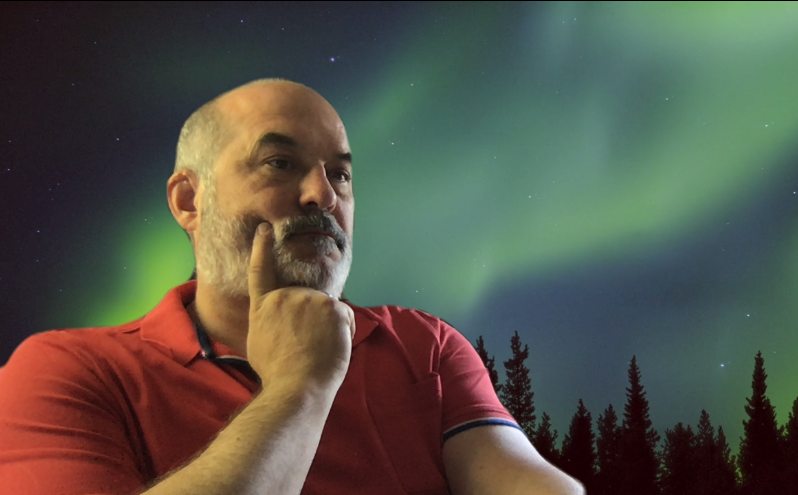
\includegraphics[width=0.9\textwidth]{Introduction_image}
	\caption{Distinction and foreground replacement of a given scenery.}
	\label{fig:Introduction_image}
\end{figure}

Figure~\ref{fig:Introduction_image} shows schematically the task. The foreground view, or every non static element in the scenery, should be located and freely dissectable from the rest of the image (background). With the help of a selectable mode parameter, the foreground and background elements will be modified accordingly and a scene will be rendred depending on the choice of the user (foreground, background, overlay, substitute)
\\

\subsection{Task Requirements}


The requirements for the program are:

\begin{itemize}

\item The program should be created in \textit{Matlab} with the help of the standard libraries and MathWorks Computer Vsion toolboxes and run with the version \textit{2020a} on \textit{Windows} and \textit{Linux} complying with a maximum running time of 30 minutes.

\item The class \textit{imagereader} should be able to read two of the three available scenerey images from a specific folder as an endless loop. The method next should deliver two tensors left and right for each selected camera accordingly and a next functionality to browse the scenery. 

\item The required function \textit{segmentation} receives the two previously created tensors left and right with successive
image pairs as input parameters, in order to create foreground and background for the first pair of pictures. This function returns a binary segmentation mask  as an output. Pixels that correspond to the
Background are assigned the value 0 and pixels that belong to the foreground get the value 1.

\item The program should be able to deal with diffrent level of scene complexity and handle the edge treatment at the transition between foreground and background.

\item Inside the function \textit{rendering} a dissection mode will be selected by the user (foreground, background, overlay, substitute) and an image will be rendered according to the mode. 

\item  Possibility of a virtual background video. 

\item Operation of the program through a user friendly graphical interface (GUI).

\end{itemize}

The algorithms and procedures used to solve the task are described in the following sections.
In the section \ref{Conception and Implementation} our procedure and the basic program flow are presented in an overview form, before the individual steps are explained in more detail in the following sections.

\subsection{Outline of the work}

This work contains theoretical fundamentals in image segmentation techniques. 
A conceptual framework of the task, will be later presented before implementing the solutions.
Additionally, the results of these methods will be compared and the limitations of each model will be discussed.
Finally, an overview of the results will be given and probable outlooks for further works will be suggested.
